%%%  Ukázkový text a dokumentace stylu pro text závěrečné (bakalářské a
%%%  diplomové) práce na KI PřF UP v Olomouci
%%%  Copyright (C) 2012 Martin Rotter, <rotter.martinos@gmail.com>
%%%  Copyright (C) 2014 Jan Outrata, <jan.outrata@upol.cz>


%%  Pro získání PDF souboru dokumentu je třeba tento zdrojový text v
%%  LaTeXu přeložit (dvakrát) programem pdfLaTeX.

%%  V případě použití programu BibLaTeX pro tvorbu seznamu literatury
%%  je poté ještě třeba spustit program Biber s parametrem jméno
%%  souboru zdrojového textu bez přípony a následně opět (dvakrát)
%%  přeložit zdrojový text programem pdfLaTeX.

%%  Postup získání Postscriptového souboru je popsán v dokumentaci.


%%  Třída dokumentu implementující styl pro závěrečnou práci. Vybrané
%%  nepovinné parametry (ostatní v dokumentaci):

%%  'master' pro sazbu diplomové práce, jinak se sází bakalářská práce

%%  'field=kód' pro Váš studijní obor, kódy pro diplomovou práci 'uvt'
%%  pro Učitelství výpočetní techniky pro střední školy a 'binf' pro
%%  Bioinformatiku, jinak je výchozí Informatika, a pro bakalářskou
%%  práci 'ainfk' pro Aplikovanou informatiku v kombinované formě,
%%  'inf' pro Informatiku, 'infv' pro Informatiku pro vzdělávání a
%%  'binf' pro Bioinfomatiku, jinak je výchozí Aplikovaná informatika
%%  v prezenční formě

%%  'printversion' pro sazbu verze pro tisk (nebarevné logo a odkazy,
%%  odkazy s uvedením adresy za odkazem, ne odkazy do rejstříku),
%%  jinak verze pro prohlížeč

%%  'biblatex' pro zapnutí podpory pro sazbu bibliografie pomocí
%%  BibLaTeXu, jinak je výchozí sazba v prostředí thebibliography

%%  'language=jazyk' pro jazyk práce, jazyky english pro anglický,
%%  slovak pro slovenský, jinak je výchozí czech pro český

%%  'font=sans' pro bezpatkový font (Iwona Light), jinak výchozí
%%  patkový (Latin Modern)

\documentclass[
%  master,
  field=inf,
%  printversion,
  biblatex,
  language=english,
%  font=sans,
  glossaries,
  theorems=false,
  sourcecodes=false,
  index
]{kidiplom}

%% Informace pro úvodní strany. V jazyku práce (pokud není v komentáři
%% uvedeno česky) a anglicky. Uveďte všechny, u kterých není v
%% komentáři uvedeno, že jsou volitelné. Při neuvedení se použijí
%% výchozí texty. Text pro jiný než nastavený jazyk práce (nepovinným
%% parametrem language makra \documentclass, výchozí český) se zadává
%% použitím makra s uvedením jazyka jako nepovinného parametru.

%% Název práce, česky a anglicky. Měl by se vysázet na jeden řádek.
\title[czech]{Vizualizace třídicích algoritmů}
\title[english]{Visualization of Sorting Algorithms}

%% Volitelný podnázev práce, česky a anglicky. Měl by se vysázet na
%% jeden řádek. Výchozí je prázdný.
%\subtitle{Ukázkový text a dokumentace stylu v \LaTeX{}u}
%\subtitle[english]{Sample text and documentation of the \LaTeX{} style}

%% Jméno autora práce. Makro nemá nepovinný parametr pro uvedení
%% jazyka.
\author{Mykhailo Klunko}

%% Jméno vedoucího práce (včetně titulů). Makro nemá nepovinný
%% parametr pro uvedení jazyka.
\supervisor{Mgr. Tomáš Kühr, Ph.D.}

%% Volitelný rok odevzdání práce. Výchozí je aktuální (kalendářní)
%% rok. Makro nemá nepovinný parametr pro uvedení jazyka.
%%\yearofsubmit{\the\year}

%% Anotace práce, včetně anglické (obvykle překlad z jazyka
%% práce). Jeden odstavec!
\annotation[czech]{Cílem práce bylo vytvořit software pro podporu výuky třídících algoritmů pomocí vizualizace průběhu třídění nejznámějšími algoritmy a jejich variantami. Program podporuje názornou vizualizaci vybraných algoritmů na zadaném či vygenerovaném vstupním poli a krokování průběhu výpočtu se souběžným zobrazením pseudokódu použitého algoritmu a aktuálních hodnot použitých proměnných.}

\annotation[english]{The main goal of the thesis was to create a teaching support software with visualization of the most known sorting algorithms and their variations. The application supports a graphic visualization of selected algorithms on randomly generated or manually created array, step-by-step execution possibility, pseudocode and current state of variables.}

%% Klíčová slova práce, včetně anglických. Oddělená (obvykle) středníkem.
\keywords[czech]{třídící algoritmus; třídění; vizualizace; výukový program}
\keywords[english]{sorting algorithm; sorting; visualization; educational software}

%% Volitelná specifikace příloh textu práce, i anglicky. Výchozí je '1
%% CD/DVD'.
%\supplements{jedno kulaté placaté CD/DVD s malou kulatou dírou uprostřed}
%\supplements[english]{one round flat CD/DVD with a small round hole in the middle}

%% Volitelné poděkování. Stručné! Výchozí je prázdné. Makro nemá
%% nepovinný parametr pro uvedení jazyka.
\thanks{I would like to acknowledge my sincere gratitude to my supervisor Mgr. Tomáš Kühr, Ph.D. for his patience and guidance throughout my bachelor thesis. Also, I would like to thank my parents for constant motivation and support from their side. Special thanks go to my friends and colleagues.}

%% Cesta k souboru s bibliografií pro její sazbu pomocí BibLaTeXu
%% (zvolenou nepovinným parametrem biblatex makra
%% \documentclass). Použijte pouze při této sazbě, ne při (výchozí)
%% sazbě v prostředí thebibliography.
\bibliography{bibliografie.bib}
%% Další dodatečné styly (balíky) potřebné pro sazbu vlastního textu
%% práce.
\usepackage{lipsum}
\usepackage{amsmath}
\usepackage{algorithm}
\usepackage[noend]{algpseudocode}
\usepackage{bm}
\usepackage{tikz}
\usetikzlibrary{calc, positioning,fit,intersections}
\usetikzlibrary{shapes.geometric, arrows}
\usepackage{forest}
\usepackage{caption}
\usepackage{subcaption}

\definecolor{mygreenii}{RGB}{34,162,70}
\definecolor{mygreeni}{RGB}{34,162,70}


%%flowchart definitions
\tikzstyle{startstop} = [rectangle, rounded corners, minimum width=3cm, minimum height=1cm,text centered, draw=black, fill=white!30] %red
\tikzstyle{io} = [trapezium, trapezium left angle=70, trapezium right angle=110, minimum width=3cm, minimum height=1cm, text centered, draw=black, fill=white!30] %blue
\tikzstyle{process} = [rectangle, minimum width=3cm, minimum height=1cm, text centered, draw=black, fill=white!30] %orange
\tikzstyle{decision} = [diamond, minimum width=3cm, minimum height=1cm, text centered, draw=black, fill=white!30] %green
\tikzstyle{arrow} = [thick,->,>=stealth]

\begin{document}
%% Sazba úvodních stran -- titulní, s bibliografickými údaji, s
%% anotací a klíčovými slovy, s poděkováním a prohlášením, s obsahem a
%% se seznamy obrázků, tabulek, vět a zdrojových kódů (pokud jejich
%% sazba není vypnutá).
\maketitle

%% Vlastní text závěrečné práce. Pro povinné závěry, před přílohami,
%% použijte prostředí kiconclusions. Povinná je i příloha s obsahem
%% přiloženého CD/DVD.

%% -------------------------------------------------------------------

\newcommand{\BibLaTeX}{\textsc{Bib}\LaTeX}

%\noindent\textcolor{red}{\LARGE Upozornění: Následující text
%  dokumentace stylu, vyjma přílohy~\ref{sec:ObsahCD}, je rozpracovaná
%  a (značně) neúplná verze!!!}

\section{Introduction}

Nowadays sorting algorithms are widely used in computer software. For example, if you open file explorer on your PC, you may see files sorted in different ways. Searching in sorted data is more efficient than in not sorted ones. Students of computer science start learning different algorithms in the first year of studies and sorting algorithms are among them.

Since I faced the problems of sorting during the course of algorithm design in the first year of my studies, there is an understanding that the visual representation is a vital part of the studying process. During working on the thesis it was very exciting to learn different techniques of sorting algorithms into the depth.

The main goal of the thesis was to create a program which would serve as a tool for understanding how most known sorting algorithms work. There was an attempt to make the best possible user experience. The demonstration software is made in a user-friendly and easy-to-use style. To gain maximal benefit from learning you can try each sorting algorithm on your data. 

The text of the thesis describes principles of the most known sorting algorithms which are demonstrated in the computer program. It might be used as a source for learning algorithms by students. Also, the program might be easily used as a demonstration by lecturers and tutors during classes. Besides, there is programmer documentation and user guide to the provided software.

Readers of this text are expected to have some programming experience to know basic data structures such as arrays, lists, trees and understand recursive procedures. Also, knowledge of some simple algorithms and their implementations could be helpful. In order to understand the topic better, knowledge of linear algebra and calculus is involved.

\newpage
\section{About algorithms}
\subsection{What is an algorithm?}

Before moving on to the main part of the text which describes algorithms and the software, we need to assure that there is an understanding of the basics. We shall begin with the algorithm definition.

What is an algorithm? How can we define it? We may say simply that an algorithm is a sequence of steps or instructions that solves some kind of problem. Although it may be a bit imprecise because we have not defined what does problem mean and what does instruction mean.

Problem is a kind of task that we need to solve. We are facing different problems every day: finding the fastest route to work or home, etc. However, not all of them are problems that may fit our algorithm definition. A suitable definition of a problem has some limitations: problem should be specified by its inputs and all inputs have to be mapped to some outputs. Step or instruction is some action that is clear to its executor. In our case, it could be a PC. To solve a problem means to find a solution for each input.

Here is more precise definition by Thomas Cormen: "Informally, an algorithm is any well-defined computational procedure that takes some value, or set of values, as input and produces some value, or set of values, as output. An algorithm is thus a sequence of computational steps that transform the input into the output." \cite{cormen}
\\\\
\textbf{5 features of an algorithm according to D. Knuth\cite{knuth1}:}
\begin{itemize}
	\item \textit{finiteness} -- an algorithm should end in a finite number of steps.
	\item \textit{definiteness} -- each step of an algorithm should have precise definition. And it means that for the same inputs we will obtain the same results.
	\item \textit{input} -- an algorithm may have inputs, they are taken from some set of objects.
	\item \textit{output} -- an algorithm may have outputs which should be in some relation with inputs.
	\item \textit{effectiveness} -- we may expect an algorithm to be effective. It means "its operations must all be sufficiently basic that they can in principle be done exactly and in a finite length of time by someone using pencil and paper."\cite{knuth1}
\end{itemize}

\subsection{Algorithm description}

To execute or understand an algorithm, we may need somehow to describe it. There are several ways of algorithm representation.

\begin{itemize}
	\item \textit{Natural language}. An algorithm described in the natural language is clear to everyone. However, it may be imprecise and somehow longer than other methods here.
	\item \textit{Programming language}. This kind of description is unambiguous. It may be used directly to create a computer program. A programming language may contain a lot of implementation details.
	\item \textit{Pseudocode} looks similar to a programming language, but it is more general, without deep details. It can be easily rewritten to most of the programming languages, and it is understandable to all programmers without regard to the exact language.
	\item \textit{Visual representation}. An algorithm may be described by many other methods, including graphical representation like flowcharts (Figure \ref{fig:flowchart}).
\end{itemize}

As an example, we will consider the algorithm for finding factorial representing it in pseudocode (Code \ref{fact}) and by the flowchart (Figure \ref{fig:flowchart}).

\begin{figure}[H]
	\begin{center}
		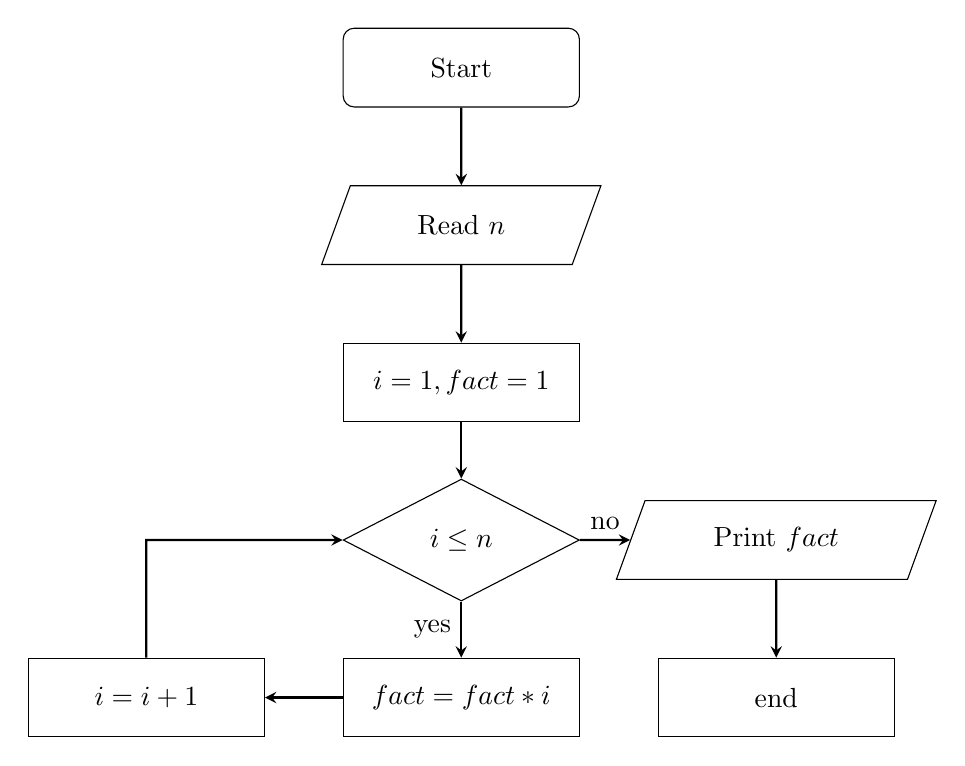
\begin{tikzpicture}[node distance=2cm]
			\node (start) [startstop] {Start};
			\node (read) [io, below of=start] {Read $n$};
			\node (setup) [process, below of=read] {$i = 1, fact = 1$};
			\node (cycle) [decision, below of=setup] {$i \leq n$};
			\node (print) [io, right of=cycle, xshift=2cm] {Print $fact$};
			\node (fact) [process, below of=cycle] {$fact = fact * i$};
			\node (i) [process, left of=fact, xshift=-2cm] {$i = i + 1$};
			\node(end) [process, below of=print] {end};		
			
			%arrows
			\draw [arrow] (start) -- (read);
			\draw [arrow] (read) -- (setup);
			\draw [arrow] (setup) -- (cycle);
			\draw [arrow] (cycle) -- node[anchor=south] {no} (print);
			\draw [arrow] (cycle) -- node[anchor=east] {yes} (fact);
			\draw [arrow] (fact) -- (i);
			\draw [arrow] (i) -- +(0, 2) -- (cycle);
			\draw [arrow] (print) -- (end);
			
		\end{tikzpicture}
	\end{center}
	\caption{Flowchart example: factorial}\label{fig:flowchart}
\end{figure}


\begin{algorithm}[H]
\caption{Factorial algorithm}\label{fact}
\begin{algorithmic}[1]
\Procedure{Factorial}{n}
\State $\textit{fact} \gets 1$
\For{ $ i \gets 1 \text{ to } n$} 
	\State $fact \gets fact * i$
\EndFor
\State \Return $fact$
\EndProcedure
\end{algorithmic}
\end{algorithm}

\subsection{Types of algorithms}

Nowadays there exists a large number of different algorithms. They are divided into different groups by different criteria. Often one algorithm may belong to several groups. Here are some of them \cite{cormen}.

\begin{itemize}
	\item \textit{Recursive algorithms} -- algorithms that call itself until the limiting condition is reached.
	\item \textit{Probabilistic algorithms} -- algorithms that make some random decisions.
	\item \textit{Parallel algorithms} -- algorithms that divide a task, for example, into threads or between processors, etc.
	\item \textit{Sequential algorithms} -- unlike the parallel algorithms, every step of the task is done in sequence.
	\item \textit{Divide and conquer} -- algorithms that divide a problem into smaller parts until they become indivisible. Then merge solutions in some way.
	\item \textit{Greedy algorithms} -- these algorithms make the best choice in a given situation. They never change their previous choice.
	\item \textit{Dynamic programming} -- algorithms that start solving a problem from the simplest to more complicated parts. They use outcomes from previous solutions.
	\item \textit{Heuristic algorithms} -- algorithms which are used for finding solution among all possible. However, there is no guarantee that a found one will be the best.
\end{itemize}

\subsection{Complexity}

Let us consider some problem that requires a solution. Then, suppose that this problem is possible to solve by three or more different algorithms. For the most suitable choice, we compare the algorithms. To compare these algorithms we need to measure the performance of each. Besides, we might need to measure the time for an algorithm to run with some input. Finally, we are moving to the concept of the algorithm complexity \citep{knuth1}, \cite{sipser}, \cite{alm2}.

There is a time complexity and a space complexity. In general, complexity gives the amount of time or space needed to run an algorithm. To be more precise: time complexity is a function $f:\mathbb{N}\to\mathbb{N}$ that maps each input to the maximum number of steps for this input needed for an algorithm to complete a task. We will be talking here only about the time complexity and will call it just complexity.

Analyzing algorithms we might want to investigate different sides of the algorithm performance. Usually, it could be a \textit{worst-case analysis} or an \textit{average-case analysis}. The worst-case analysis implies determining the longest running time of all inputs with the same length. In the average-case analysis, we take the average running time of inputs with the same length.

Often complexity of an algorithm is measured on the large inputs. Since complexity is expressed by a polynomial, we might want to have it in a more convenient form. This type of estimation is called an \textit{asymptotic analysis}. Such form takes only the highest order term of the polynomial.

To be more clear, let us have an example. $f(n) = 5n^3 + 10n^2 + 20n + 4$, the highest degree term here is $5n^3$. In some cases we can omit the coefficient 5, now $f$ is asymptotically at most $n^3$.

For such approximations there exist different notations \cite{knuth1}, \cite{sipser}:

\begin{enumerate}
	\item \textit{Asymptotic upper bound} (or Big O notation). For the function $f(n)$ with an input size of $n$, $O(f(n))$ means that the running time or complexity of an algorithm grows as much as the $f(n)$ but may grow more slowly. It represents a worst-case complexity. Sometimes we may write $f(n) = O(g(n))$. To be more precise, it means that there exists some constant $c > 0$ such that $f(n) \leq c * g(n)$ for some large enough $n$ (Figure \ref{fig:big-omega}).
	\item \textit{Asymptotic lower bound} (or Big Omega notation). If the complexity of some algorithm is in $\Omega(f(n))$, it means that there exists some large enough $n$ such that the function $f(n)$ is a lower bound for the algorithm running time. It represents the best-case complexity. $f(n) = \Omega(g(n))$ means that there exists some constant $c > 0$ such that $c * g(n) \leq f(n)$ for some large enough $n$.
	\item \textit{Asymptotic tight bound} (or Big Theta notation). This notation combines both lower and upper bounds. This way, it shows an average-case complexity.
\end{enumerate}

All the functions that we have here we will assume to take only non-negative values. Also, there is a \textit{small o} notation. It slightly differs from the \textit{Big O} notation. "Big-O notation says that one function is asymptotically no more than  another. To say that one  function is asymptotically less than another we use small-o notation."\cite{sipser}

\begin{figure}[H]
	\begin{center}
		\begin{tikzpicture}
			\draw[->]  (0,0)coordinate(O) -- (7,0) node[anchor=north] {$n$};
			\draw[->]  (0,0) -- (0,6);
			\draw[domain=0:7,smooth,variable=\x,black,name path=c1] plot ({\x},{0.5*\x+1*sin(\x r)+1})node[right]{$c * g(n)$};
			\draw[domain=0:7,smooth,variable=\x,black,name path=c2] plot ({\x},{0.2*\x+0.5*sin(\x r)+1.5})node[right,black]{$f(n)$};
			\fill[red,name intersections={of=c1 and c2}] (intersection-1) circle (2pt);
			\draw[dashed] (intersection-1) -- (intersection-1|-O) node[below]{$n_0$};

		\end{tikzpicture}
		\caption{$f(n)$ in $O(g(n))$} \label{fig:big-omega}
	\end{center}
\end{figure}

For the asymptotic analysis of an algorithm mostly the worst-case complexity is used. Algorithm is considered for practically solvable if its running time is in $O(n^c)$, $c$ is usually a small constant \cite{cormen}. 

Here are some complexities (from the slowest to the fastest growing):
\begin{enumerate}
 \item $O(1)$ -- constant complexity
 \item $O(\log(n))$ -- logarithmic
 \item $O(n)$ -- linear
 \item $O(n \log(n))$ -- linear-logarithmic
 \item $O(n^2)$ -- quadratic
 \item $O(2^n)$ -- exponential
 \item $O(n!)$ -- factorial
\end{enumerate}

\subsection{Sorting}

As was already said that sorting is used for solving a wide range of problems. It may be used for further searching or, for example, as part of different complex tasks. We were talking about sorting. But what actually sorting is?

Simply said, sorting is a process of rearranging of items, which are possible to compare, in ascending or descending order. In the text we are meaning only ascending order if not stated in a different way.

Ascending order means that items in a sequence are arranged from the smallest to the largest item. On the contrary, descending order means positioning from the largest to the smallest item.
\\\\
Sorting algorithms are divided into two main types \citep{alm2}:
\begin{enumerate}
	\item \textit{Algorithms of internal sorting} -- all the data to sort is stored in the internal memory during the sorting process. It is used when the amount of data to sort is known.
	\item \textit{Algorithms of external sorting} -- all the data to sort is stored outside the internal memory (e.g. on a hard disk). These algorithms usually combine sorting in the internal memory, merging of sorted parts and saving them to the external memory.
\end{enumerate}

In the text we are talking only about the algorithms of internal sorting. Here are five main techniques which are usually used and algorithms which use these techniques and are included in the software \cite{knuth3}:
\begin{enumerate}
	\item \textit{Sorting by Insertion} -- single items from the sequence are put into the right place of the sorted part. Here belongs \hyperref[sec:insertion]{Insertion Sort}.
	\item \textit{Sorting by Exchanging} -- swap elements of each pair that are out of order till no more such pairs exist. Here we have \hyperref[sec:bubble]{Bubble Sort}, \hyperref[sec:cocktailsort]{Cocktail Sort}, \hyperref[sec:quicksort]{Quick Sort}.
	\item \textit{Sorting by Selection} -- method that uses repeated selection. \hyperref[sec:selection]{Selection Sort} and \hyperref[sec:heapsort]{Heap Sort} use this technique.
	\item \textit{Sorting by Merging} -- merging smaller parts with the right order. And \hyperref[sec:mergesort]{Merge Sort} uses it. 
	\item \textit{Sorting by Distribution} -- technique which does not use comparisons to sort. It works relying on the knowledge about the set from where data to sort is taken. Data is distributed to some intermediate structures according to values. \hyperref[sec:radixsort]{Radix Sort}, \hyperref[sec:bucketsort]{Bucket Sort} and \hyperref[sec:counting]{Counting Sort} belong here.
\end{enumerate}

\newpage
\section{Sorting algorithms}

This section describes algorithms represented in the program.

\subsection{Insertion Sort}
\label{sec:insertion}
Insertion Sort algorithm has a simple idea. Assume an array with items to be sorted. We divide the array into two parts: sorted one and unsorted one. At the beginning sorted part consists of the first element. Then, for each item that we have in the unsorted part, we take element and insert it into the right place among the sorted items.

\begin{figure}[H]
\begin{center}
	
	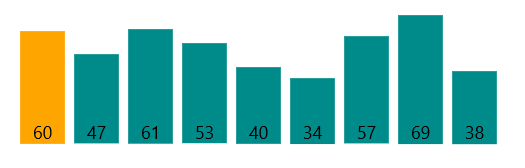
\includegraphics[scale=0.7]{img/Insertion.png}
	\caption{Insertion Sort: sorted and unsorted parts at the beginning}\label{fig:insert}
\end{center}
\end{figure}

In order to insert element into the right place in the sorted part, we compare selected item from the unsorted part with each item from the sorted part in the direction from right to left. Comparing continues until smaller or equal element is found or no elements to compare left. After each comparison, if current item in the sorted part is greater, we move that current item one position right. Finally, when the right position is found, we insert an item into the sorted part. Complexity of Insertion Sort is $\Theta(n^2)$.

\subsection{Selection Sort}
\label{sec:selection}

Selection Sort algorithm is based on the repeated selection. Here we consider finding minimal key from the unsorted part and swapping it with the first unsorted key. As well as in the \hyperref[sec:insertion]{Insertion Sort}, sorted part grows from the beginning of the sequence.

Assume an array of items to sort. At the beginning of the sorting process unsorted part is represented by the whole array. Then, the first item of the unsorted part is set as the smallest item and is compared with the follow-up elements. When smaller item is found, it is set as a new smallest key. After the end of the array is reached the smallest item is swapped with the first element of the unsorted part and it becomes the sorted part of the array. This step is repeated till the array is sorted. Complexity of this sorting algorithm is $\Theta(n^2)$.

\subsection{Bubble Sort}
\label{sec:bubble}
Bubble Sort is based on the idea of exchanging two adjacent elements if they have wrong order. The algorithm works stepping through all elements from left to right, so the largest elements tend to move or "bubble" to the right. That is why the algorithm is called Bubble Sort.

Now we are going to the details. Let us have an unsorted array. The algorithm does iterations through the unsorted part which is the whole array at the beginning. And with each iteration through the array the range of inspected items is decreased by one till only two elements left. After this two elements are compared and possibly swapped, the array is considered as sorted.

Bubble Sort complexity is $\Theta(n^2)$.

\begin{figure}[H]
\begin{center}
	
	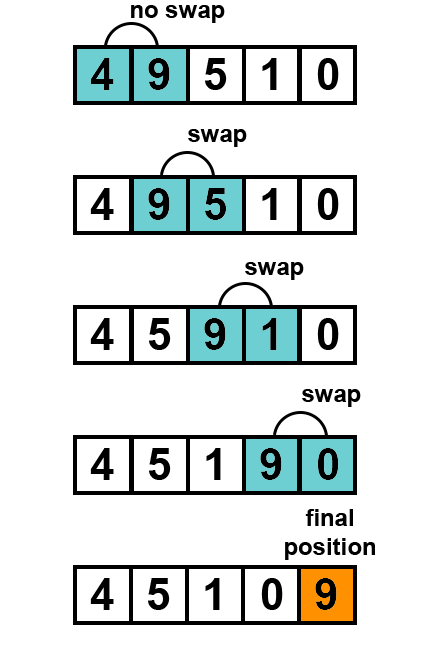
\includegraphics[scale=0.7]{img/Bubblesort.png}
	\caption{Bubble Sort in progress}\label{fig:bubble}
\end{center}
\end{figure}

%add pic of bubblesort in action
\subsection{Cocktail Sort}
\label{sec:cocktailsort}

Cocktail Sort or also known as Bidirectional Sort. This algorithm similarly to the Bubble Sort uses the idea of exchanging unordered adjacent items of array. 

Assume array that needs to be sorted in ascending order. Above we described Bubble Sort and this algorithm has a significant problem. It iterates through array only in one direction. This way, smaller items which are closer to the end of array reach its right positions slowly.

The solution is to make Bubble Sort iterate left-to-right and right-to-left. Cocktail Sort uses two cycles inside a big one. Here $a$ and $b$ are the positions of the leftmost and the rightmost elements of the array.

The way the algorithm works:

\begin{enumerate}
 \item Iterate from $a$ to $b$, compare adjacent elements and swap if they are not ordered.
 \item Iterate from $b$ to $a + 1$ same way as in the step $1$
 \item Repeat steps 1. and 2. but with a bit different range from $a = a + 1$ to $b = b - 1$
\end{enumerate}

For Cocktail Sort worst case complexity remains $\Theta(n^2)$.

\subsection{Quick Sort}
\label{sec:quicksort}
Quick Sort works on the principle "divide and conquer". It recursively applies itself on smaller parts of array until it is not sorted.

Algorithm takes one item at unsorted array or its part, usually it is the leftmost or the rightmost element of array. Then this item, also known as pivot, is moved to its final position in the array that is should occupy. While determining pivot's position, other elements of array are rearranged the way that no bigger elements on the right and no smaller elements are on the left.

This way, it is enough to apply Quick Sort on each part of array not including pivot until array is not sorted.

\begin{figure}[H]
\begin{center}
	
	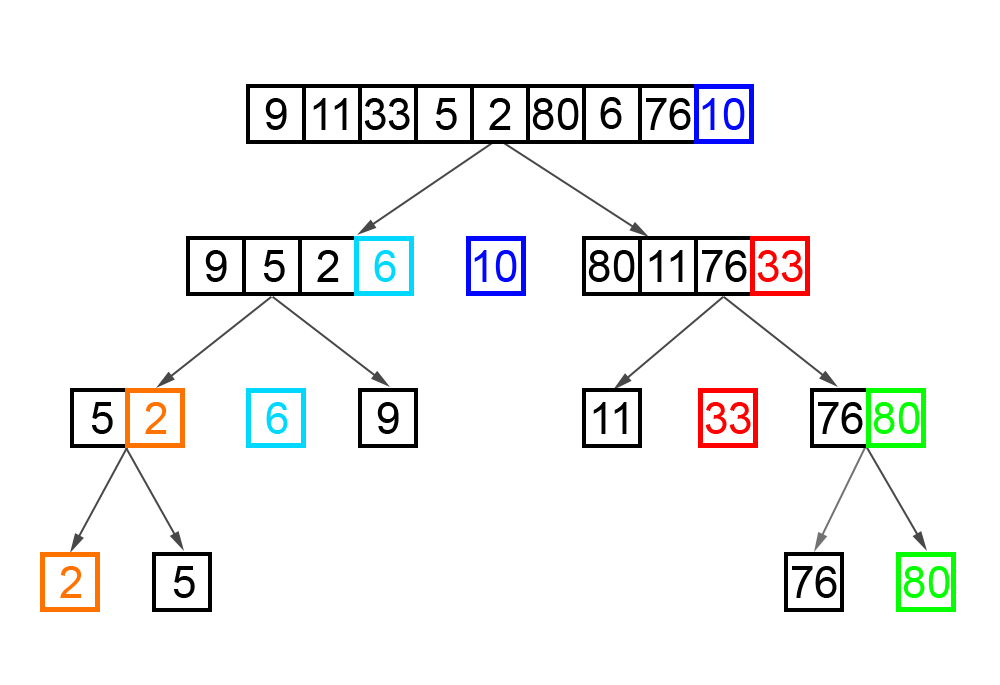
\includegraphics[scale=0.35]{img/Quicksort.png}
	\caption{Quick Sort principle}\label{fig:insert}
\end{center}
\end{figure}

There are several methods of partitioning of array into two parts, here I want to describe one that is demonstrated in the software part of this work.

Firstly, a pivot and index item are selected on the unsorted array or its part. Assume pivot is the rightmost item and index is the first. Next, each item of the array except pivot is compared with the pivot. If a current item is less or equal to the pivot, it is swapped with the index item, next in order item becomes an index. Finally, index and pivot are swapped and this way pivot is on its final position.

Quick Sort is counted as an effective algorithm because its average complexity is $\Theta(n \log n)$. However, when array is maximally unbalanced it may show worst performance. Worst case complexity is $\Theta(n^2)$.

\subsection{Merge Sort}
\label{sec:mergesort}

Merge Sort as well as \hyperref[sec:quicksort]{Quick Sort} is an algorithm of type "divide and conquer". Its logic is simple: divide data into two parts, sort the left part, sort the right part, then "merge" the parts back.

The algorithm works by the recursive application itself on the unsorted parts. In the beginning, it selects the middle item, which becomes the rightmost element of the left part. Then, it recursively sorts both parts. Finally, the algorithm "merges" two sorted parts. Merging procedure itself takes items from each of two sorted parts one by one, compares them and moves the smallest to the output, repeats the previous step. Merge Sort complexity is $\Theta(n \log n)$

\begin{figure}[H]
\begin{center}
	
	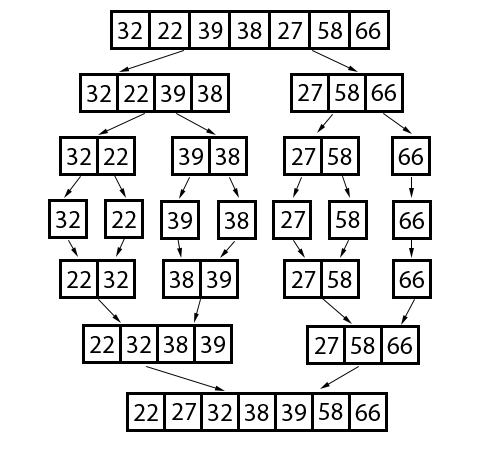
\includegraphics[scale=2.5]{img/Mergesort.png}
	\caption{Merge Sort principle}\label{fig:insert}
\end{center}
\end{figure}

\subsection{Heap Sort}
\label{sec:heapsort}

Heap Sort is a selection based algorithm and it offers another interesting approach to sorting. In comparison with the \hyperref[sec:selection]{Selection Sort} it has optimized selection by using binary heap data structure.

Binary heap is a complete binary tree; it means that all levels of tree, except the last one, must be completely filled with nodes. Also, this data structure satisfies the \textit{heap condition}: each node key is greater than or equal to its child keys (this heap type is called \textit{max-heap}).

\begin{figure}[H]
\begin{center}
	
	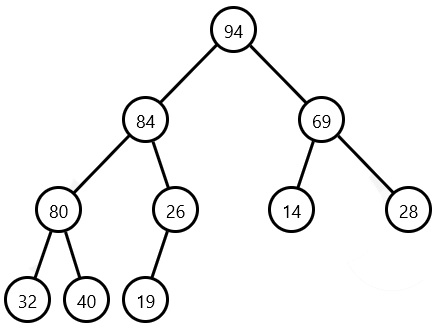
\includegraphics[scale=0.7]{img/Maxheap.png}
	\caption{Max-Heap}\label{fig:maxheap}
\end{center}
\end{figure}

Binary heap may be implemented by simple array. Item at position zero is a root node, items at position one and two are respectively left and right children of the root. From that representation it is easy to find children of each node (if they exist). Assume a node at position $k$ then its left child is at $2k + 1$ and its right child is at $2k + 2$.

\begin{figure}[H]
\begin{center}
	
	
\includegraphics[scale=3]{img/Heapsort.png}
	\caption{Children positions in heap}\label{fig:heapsort}
\end{center}
\end{figure}

\textbf{Heap Sort itself works as follows:}
\begin{enumerate}
 \item \label{itm:step1} Build max-heap
 \item \label{itm:step2} Swap root and the last node, reduce size of heap by one
 \item \label{itm:step3} Build max-heap without the nodes on a reduced position
 \item Repeat steps \ref{itm:step2} and \ref{itm:step3} until the range of array is one
\end{enumerate}

To build \textit{max-heap} from current node we need to assure that right and left children comprise max-heaps. This way, in the first step procedure for building max-heap is recursively applied for each node that has at least one child from bottom to top.

After each swap of the root node and the node at last considered position, the last node takes its final place. This way it joins the sorted part of an array. Worst and average case complexity of Heap Sort are both $\bm{\Theta(n \log(n))}$.

\subsection{Counting Sort} 
\label{sec:counting}

Counting Sort is usually used for sorting integer keys in the range from $0$ to $k$. The algorithm is based on counting keys of distinct values. Final positions of keys are calculated from the previous computations. It means that the position of some key $x$ depends on the count of keys that are less than $x$.

For better understanding let us have an example. Assume we have integers in the range from $0$ to $k$ and an empty output array. For this range, we create helping array that will keep counters for each number from the range. Then all counters from the helping array are set to $0$. To obtain final positions for items to be sorted we need to make further computations.

Firstly, for each element from the initial array, we increase the respective counter which is determined from the element value. That means the value of the element is its counter position in the helping array. Secondly, we need to sum each counter with previous. Finally, for each item from the initial array, the respective counter is decreased by one, and the value of counter now is the final position, we move the item to the output array.

Worst case complexity for Counting Sort is $\Theta(k + n)$, where $k$ is number of items in range and $n$ is size of array to be sorted.

\subsection{Radix Sort}
\label{sec:radixsort}

The Radix sorting algorithm is based on the idea of using separate digits to determine final number positions. It works with the help of some stable sorting algorithm, for example \hyperref[sec:counting]{Counting Sort}, taking digits one by one from least significant to most significant.

For better understanding let us go to the details. Assume the array of integers. Let $d$ be the number of digits of the largest item from the array. If there are numbers from the array that have less count of digits than the $d$ is, then insufficient digits are counted as digits with zero values.

This way, for each digit from least significant to most we sort the input array according to the current digit (Figure \ref{fig:radixsort}). Here we use \hyperref[sec:counting]{Counting Sort} or another stable algorithm.

\begin{figure}[H]
\begin{center}
	
	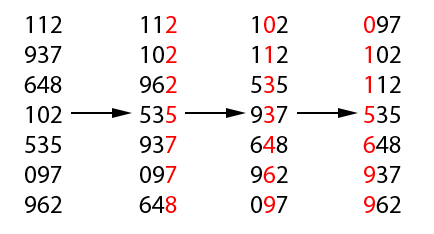
\includegraphics[scale=2]{img/Radixsort.png}
	\caption{Radix Sort principle}\label{fig:radixsort}
\end{center}
\end{figure}

\subsection{Bucket Sort}
\label{sec:bucketsort}

Bucket Sort, as well as \hyperref[sec:counting]{Counting Sort}, requires data in a known range with a uniform distribution over this range.

In the beginning, the algorithm creates n intervals of the same size. For each interval, it creates a dynamic structure which will hold items from the input. These dynamic structures are called buckets.

Firstly, Bucket Sort distributes data to buckets. Then, it sorts each non-empty bucket. For this task, we can use, for example, \hyperref[sec:insertion]{Insertion Sort}. Finally, the algorithm moves items from each bucket one by one to the output array. 

In case we select Insertion Sort as the algorithm for sorting buckets, the worst case complexity for Bucket Sort is $\Theta(n^2)$. However, the average case complexity is $\Theta(n)$.

\begin{figure}[H]
\begin{center}
	
	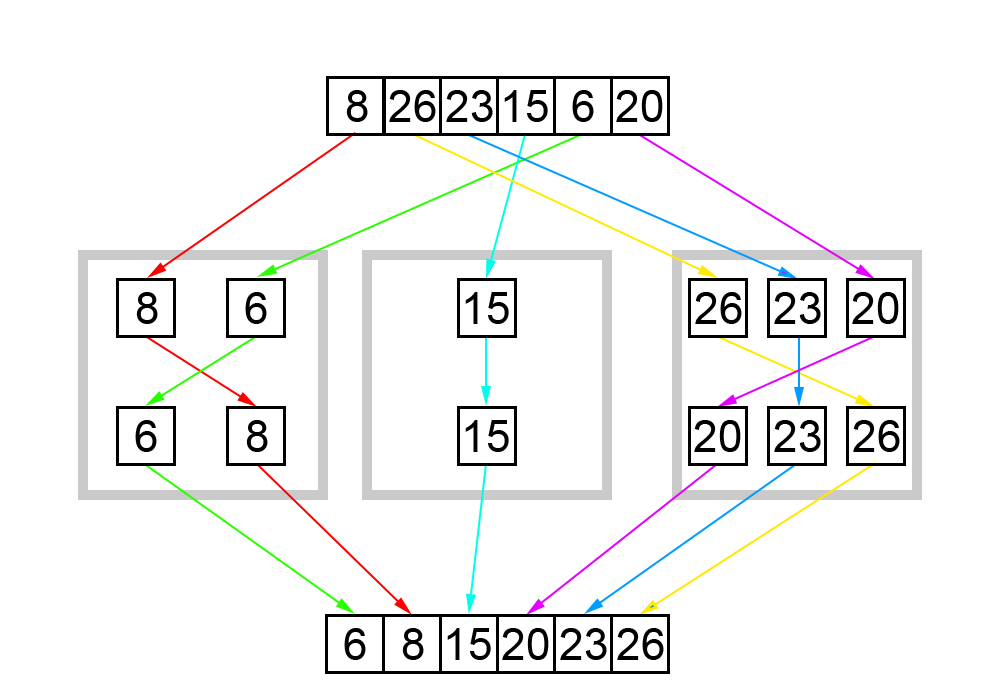
\includegraphics[scale=0.3]{img/Bucketsort.png}
	\caption{Bucket Sort principle}\label{fig:bucketsort}
\end{center}
\end{figure}

\newpage
\section{Documentation}

This section describes the structure of the program and some useful topics from the programmer's side. 

\subsection{Used technologies}

Nowadays there are a lot of programming languages, libraries, frameworks. On the one hand, a software developer has a wide choice. On the other hand, here comes up a new problem to make the right choice which should fit the best to the current task.

The main programming language of the thesis software is Java\footnote{\href{https://docs.oracle.com/javase/tutorial/getStarted/intro/definition.html}{Java}}. To be more precise, Java Platform, Standard Edition 8. Java is a cross-platform, object-oriented language. Its motto is "write once, run anywhere". It means that compiled java application runs on all platforms, that are supported by Java. Java applications are compiled to the kind of bytecode and may be running on the \Gls{JVM}\footnote{\href{https://www.geeksforgeeks.org/jvm-works-jvm-architecture/}{What is JVM}} regardless of the platform. 

As for the visual side of the application, Java provides a good JavaFX\footnote{\href{https://docs.oracle.com/javase/8/javafx/get-started-tutorial/jfx-overview.htm}{JavaFX overview}} library which is enough for the purpose. Here JavaFX was used both for the user interface and algorithms visualization. Also, JavaFX provides the possibility of using \Gls{CSS}. The visualization software uses \Gls{CSS}\footnote{\href{https://www.w3schools.com/css/default.asp}{About CSS}} for styling some elements of the user interface.

The project was created and developed in the NetBeans IDE, although you may use other IDEs that support importing the NetBeans projects. It was developed under the Windows operating system and was tested with different resolutions and on the macOS. A version control system Git\footnote{\href{https://git-scm.com/}{Learn and download Git}} in connection with the GitHub was used. All the working steps of the project you may follow on \href{https://github.com/klnmi97/Sorting-Visualization}{the GitHub website}.

\newpage
\subsection{Structure overview}

Program source codes are structured into packages:
\begin{figure}[H]
	\begin{flushleft}
		\begin{forest}
			for tree={
    		font=\sffamily,
    		text=white,
    		text width=3.5cm,
    		minimum height=0.5cm,
    		if level=0
    		  {fill=mygreenii}
    		  {fill=mygreeni},
    		rounded corners=4pt,
    		grow'=0,
    		child anchor=west,
    		parent anchor=south,
    		anchor=west,
    		calign=first,
    		edge={mygreenii,rounded corners,line width=1pt},
    		edge path={
    		  \noexpand\path [draw, \forestoption{edge}]
    		  (!u.south west) +(7.5pt,0) |- (.child anchor)\forestoption{edge label};
		    },
    		before typesetting nodes={
      		if n=1
        		{insert before={[,phantom]}}
        		{}
    		},
    		fit=band,
    		s sep=10pt,
    		before computing xy={l=15pt},
  		}
		[sortingvisualization
		  [Constants]
  		  [Controllers]
		  [Data]
		  [Enums]
		  [NodeControllers]
		  [UI]
		  [Utilities]
		  [Algorithms]
		]
		\end{forest}
		%\captionsetup{justification=raggedright, singlelinecheck=false}
		%\caption{Project structure}\label{fig:structure}
	\end{flushleft}
\end{figure}

Each package contains certain classes, which are grouped by the purpose of use. Next subsections contain some general descriptions of the classes from packages. 
\subsubsection{A root package}
The root package contains only one class. It is MainUI.java. This class serves as the main class which starts the application. Although JavaFX provides the possibility of using XML-based language for creating a user interface, here it is not used. The MainUI class defines main user interface elements and does the instantiating of controllers.

\subsubsection{Constants, Data and Enum packages}
All these three packages work with data and data structures, although a bit differently. Constants package has only an eponymous class. This class contains final static variables that are used as default values in the program. Data package contains classes which serve as definitions for data objects. \textit{BindingData} class instance holds data for control buttons bindings. Results class defines object that is used for transferring results from the input dialog. Enum package contains one definition of the enum class. \textit{Algorithm} enum defines list of algorithms that are visualized in the program. For example, a list with algorithm names in the main window is generated from this enum.

\subsubsection{Controllers package}
The package has two Java class files: \textit{AnimationController.java} and \textit{ViewController.java}. The first one is responsible for the control of animations run. And the second one controls the graphic part of the application: creation the right graphic representation of array nodes, control of animation creation, pseudo code creation control. Both are used in the main class.

\subsubsection{NodeControllers package}
NodeControllers package includes \textit{BrickNode.java, ColorInfoManager.java, DynamicNodes.java, FixedNodes.java, Pseudocode.java, Tree.java and Vari\-ables\-Info.java}.

BrickNode class defines kind of representation of the key from the array. After instantiating it can be styled in many ways. This is done by the different node managers. We shall talk about them next. Before moving on, we describe node managers generally. These objects are responsive for creation a visual representation from the given data. Also, they may create some additional graphic items, e.g. buckets for the Bucket Sort. Node managers define animations for the certain types of nodes and define their own metric system for certain type of nodes.

The first is \textit{DynamicNodes} class. \textit{DynamicNodes} object manages visual nodes whose height depends on their value. Then, there is \textit{FixedNodes} class. This node manager class defines a manager that controls nodes of fixed size. Finally, there is \textit{Tree} node manager. \textit{Tree} represents manager that creates and controls a visual binary heap. 

\begin{figure}[H]
	\begin{subfigure}{0.31\textwidth}
		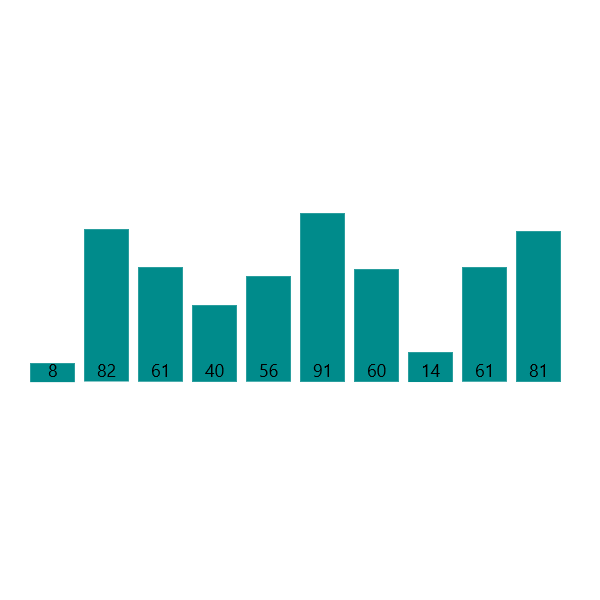
\includegraphics[width=\linewidth]{img/dynamic.png}
		\caption{Dynamic-size nodes} \label{fig:1a}
	\end{subfigure}
	\hspace*{\fill} % separation between the subfigures
	\begin{subfigure}{0.31\textwidth}
		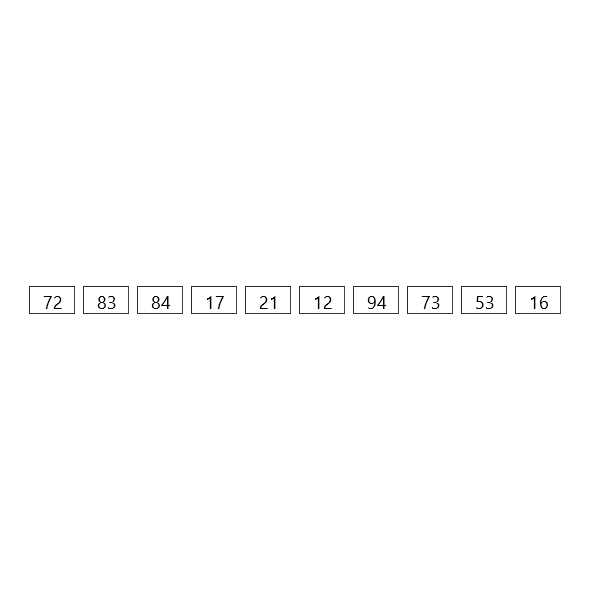
\includegraphics[width=\linewidth]{img/fixed.png}
		\caption{Fixed-size nodes} \label{fig:1b}
	\end{subfigure}
	\hspace*{\fill} % separation between the subfigures
	\begin{subfigure}{0.31\textwidth}
		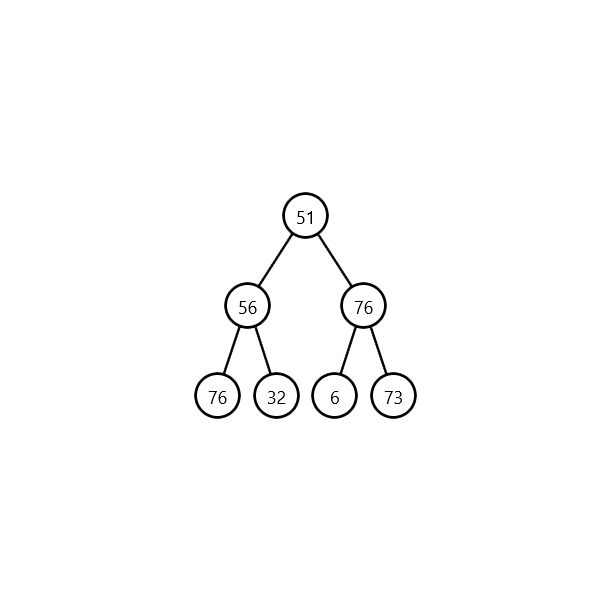
\includegraphics[width=\linewidth]{img/tree.png}
		\caption{Tree nodes} \label{fig:1c}
	\end{subfigure}
	\caption{Node types} \label{fig:1}
\end{figure}

%%add about pseudocode
\textit{Pseudocode} class, as it is clear from the title, defines a manager that controls the creation and animating of the pseudocode that appears on the information side panel. \textit{VariablesInfo}, in turn, defines another dynamic part of the information side panel, that shows current details during the visualization process and state of some variables. \textit{ColorInfoManager} represents information about the meaning of single colors of nodes. Usually, a description is shown for the dynamic type of nodes which tend to change their colors.

\subsubsection{UI package}
UI or user interface package includes different additional classes that define additional parts of the graphic user interface. There are \textit{InfoDialog} which represents dialog that shows short descriptions of individual algorithms. \textit{InputDialog} instance accepts user input data. \textit{Toast} is a help message in Android OS style.

\subsubsection{Utilities package}
The Utilities package contains different kinds of tools. \textit{ArrayUtils} is a supporting tool while working with an array. \textit{DescriptionReader} is a tool for reading algorithm description from a file. \textit{Scaling} class defines a tool that counts the scaling factor to fit different screens.

\subsubsection{Algorithms package}
And the last, but not the least significant, package called Algorithms. It contains classes that actually do animating of the algorithms. Each class that creates animations is supposed to extend \textit{Sorting} class and implement the \textit{AbstractAlgorithm} interface. List of class definitions here corresponds to the list of algorithms in the \textit{Algorithm} enum.

\subsubsection{Resources}
Apart from the source code packages, project has a resource folder inside. This folder contains images that are used in the program: icons, button images. Also, it includes \Gls{CSS} files that are used for the styling of the main window (style.css) and of the input dialog (dialog.css).

In the resource folder exists a subfolder that stores files with descriptions of the algorithms. File names here correspond to the long names from the \textit{Algorithm} enum without spaces. Such name conventions help the reader tool to find the right description.

\newpage
\section{User Guide}

\subsection{System requirements}

Since Java is cross-platform, you may use the application within the most popular PC operating systems where Java is supported. Here are given minimal system requirements for several operating systems.

\noindent \textbf{Requirements:}
\begin{itemize}
	\item Operating system: minimum Windows XP SP3 or Mac OS X 10.4.10 or Ubuntu 8.04 
	\item Java: Java SE 8 with minimum update 40 (8u40) or update 51 (8u51) in case of Windows 10 operating system
	\item Processor: Dual-Core processor, 1.8 GHz
	\item Memory: 512MB of RAM (1GB recommended)
\end{itemize}

\subsection{Starting application}

Since Java applications are not native applications to the most popular operating systems for PC, you need to have JDK\footnote{\href{https://www.oracle.com/technetwork/java/javase/jdk-8-readme-2095712.html}{Java Development Kit}} or JRE\footnote{\href{https://www.w3schools.in/java-tutorial/jre/}{Java Runtime Environment}} installed and configured. In case it is already done, it is enough to run the file of the application with \textit{.jar} extension as simple application.

Also, it is possible to use option "Open with". Here is necessary to select the right application. For example, in the Windows operating system it is usually "Java(TM) Platform SE binary" or \textit{javaw.exe}.

Next opportunity is to run it through the command line. For Windows and macOS it is done the same way. Type the command from below and add the right path before the file name. 
\begin{lstlisting}
java -jar Sorting-Visualization.jar
\end{lstlisting}

Just after running the application, the main window (Figure \ref{fig:ui}) shows up and the application is ready to use.

\subsection{User interface}

As it was stated above, the main aim of the application is to be as much user-friendly as possible. This part describes the user interface of the application.

Main window (Figure \ref{fig:ui}) consists of the visualization panel (1), information panel (2), control panel (3) and upper panel (4).

\begin{figure}[H]
\begin{center}
	
	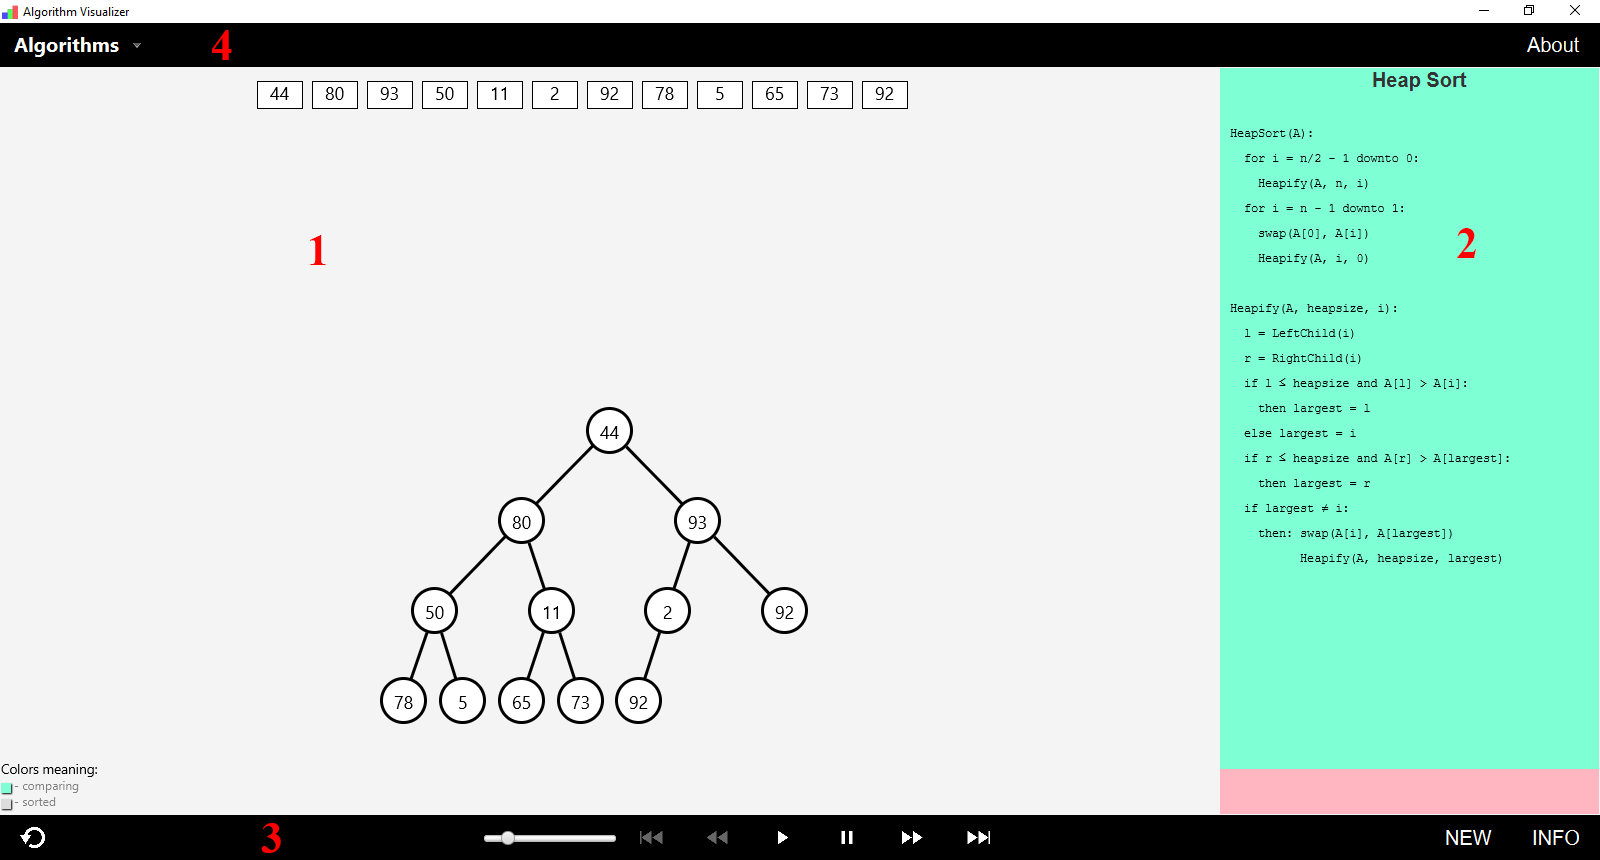
\includegraphics[width=\textwidth]{img/UI.png}
	\caption{Main window}\label{fig:ui}
\end{center}
\end{figure}

\subsubsection{Visualization panel}
Visualization panel (Figure \ref{fig:vispanel}) is the main space for the visualization of algorithms. It shows different types of nodes which represent array items. Animated movements of these nodes show individual steps of a sorting algorithm. 

For some algorithms, there is a description of the node colors available. It is located in the bottom left corner.

\begin{figure}[H]
\begin{center}
	
	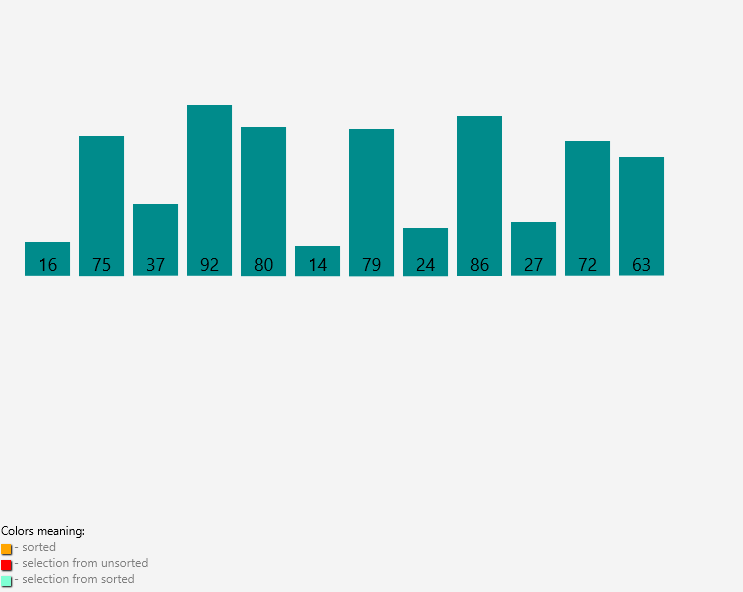
\includegraphics[scale=0.4]{img/ui/Vispanel.png}
	\caption{Visualization panel}\label{fig:vispanel}
\end{center}
\end{figure}

\subsubsection{Control panel}

Control panel gives a user the possibility to have full control over the algorithm visualization process. It is possible to run visualization, to pause it, even to go through step by step forth and back. If you do not understand what the exact button means, hover the mouse cursor over some active button and you will see a tip.

Buttons and other interactive elements on the panel (Figure \ref{fig:controls}, from left to right) are "Reset", "Animation speed slider", "Go to start", "Step back", "Play", "Pause", "Step forth", "Go to end", "New" and "Info".

\begin{figure}[H]
\begin{center}
	
\includegraphics[scale=0.5]{img/ui/Controls.png}
	\caption{Control panel}\label{fig:controls}
\end{center}
\end{figure}

"Reset" action creates a new sorting visualization of the current algorithm with a randomly generated array. "New" action allows a user possibility to enter custom data. "Info" opens a window with a description of the current algorithm.

\subsubsection{Information panel}

The information panel (Figure \ref{fig:infopanel}) is located on the right side of the window. It consists of the header with the name of the current algorithm, the pseudocode of the selected algorithm and description of the current state.

During the run of the visualization, this information is dynamically updated according to the current algorithm. Application synchronously highlights used lines of code and updates the current state line showing the current state of the algorithm and some values of used variables.

\begin{figure}[H]
\begin{center}
	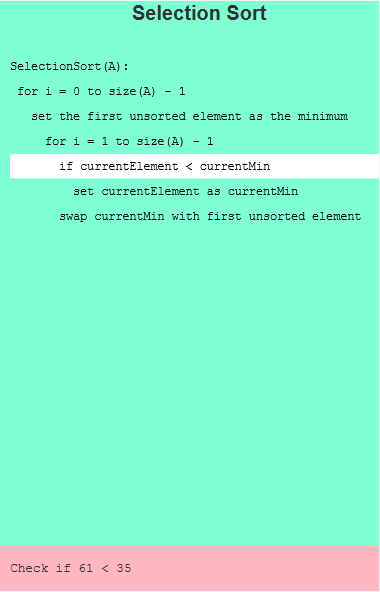
\includegraphics[scale=0.4]{img/ui/Infopanel.png}
	\caption{Information panel}\label{fig:infopanel}
\end{center}
\end{figure}

When the window is resized and the information panel does not fit, it becomes scrolable. It is possible to hide this panel by clicking on it. In order to restore the panel, use the button with arrow which is located on the place of the side panel.

\subsubsection{Upper panel}
The upper panel includes selector of the algorithms. To see the list of available algorithms click on the "Algorithms" (Figure \ref{fig:selector}).

\begin{figure}[H]
\begin{center}
	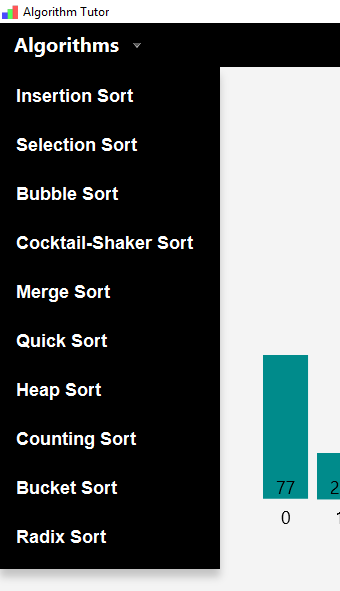
\includegraphics[scale=0.3]{img/ui/Selector.png}
	\caption{Algorithm selector}\label{fig:selector}
\end{center}
\end{figure}

\subsection{Interaction}

This section describes possible interactions between user and application.

\subsubsection{Starting new visualization}
To start a new visualization, there are some options. You may either start it by selecting an algorithm from the algorithm selector on the upper panel or click "Reset" to initialize new visualization of the current algorithm with random data. Finally, a user can initialize new visualization with custom data.

\begin{figure}[H]
\begin{center}
	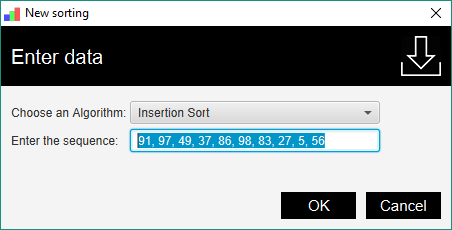
\includegraphics[scale=0.5]{img/ui/WindowNew.png}
	\caption{Window "New sorting"}\label{fig:new}
\end{center}
\end{figure}

To initialize new visualization with custom data, click the "NEW" button. After it, there appears a window (Figure \ref{fig:new}). To select an algorithm, choose one from the drop-down list. The input field, which is a line lower, allows a user to enter a sequence of integers. By default, it is filled with randomly generated numbers. For separation of numbers use space or comma. The input field accepts numbers from range 0 - 99, except a pair of algorithms. Counting Sort has range 0 - 9 and Radix Sort accepts numbers from range 0 - 9999. 

\subsubsection{Visualization control}

After setting up a new visualization, it is easy to control sorting visualization flow. To run sorting visualization click on the "Play" button or press \textbf{R} key. "Play" button may not be available in case visualization is already running or is finished. Also, "Play" button resumes sorting process after it was paused. The process is paused by pressing "Pause" button.

Stepping through the sorting process is performed by two buttons. Step back action is done by clicking the "Step Back" button, which is to the left of the "Play" button. Step forth is made by clicking the "Step Forth" button, which is to the right of the "Pause" button. Both actions are not possible during sorting is running.

In addition, there are buttons that allow go to the beginning and to the end. "Go to start" returns sorting in the initial state. "Go to end" action is intended to fast-forward visualization to the "sorted" state.

Finally, the application allows for changing the speed of visualization. By default, there is an optimal speed for animation flow. To slow down animations, move the knob to the left. To make the visualization run faster, slide knob to the right.

\subsubsection{Information about the application}

To display a window with information about the application (Figure \ref{fig:about}) click the "About" button on the upper panel or press \textbf{F1} key.

\begin{figure}[H]
\begin{center}
	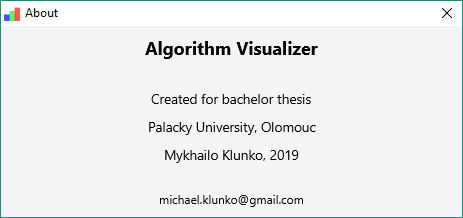
\includegraphics[scale=0.7]{img/ui/WindowAbout.PNG}
	\caption{Window "About"}\label{fig:about}
\end{center}
\end{figure}

\subsubsection{Opening description}

There is a short description for each algorithm. To show information click "Info" button on the control panel or press \textbf{F2}. Then a window with the short description will show up (Figure \ref{fig:desc}). To close the window use standard close button or press \textbf{Esc}.

\begin{figure}[H]
\begin{center}
	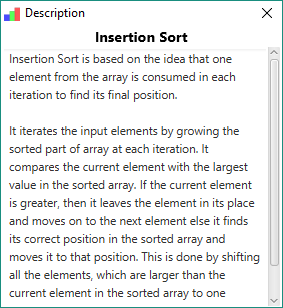
\includegraphics[scale=0.7]{img/ui/WindowDescription.png}
	\caption{Window "Description window"}\label{fig:desc}
\end{center}
\end{figure}

\subsubsection{Escaping application}

Close application by clicking exit button. Its location depends on the operating system. Also, you may use the \textbf{Esc} button.

\subsection{Keyboard shortcuts}

Keyboard shortcuts for Windows and macOS.

\begin{table}[H]
	\centering
	\caption{Shortcuts}\label{tab:keyboard}
	\begin{tabular}{||l|l|l||}
	\hline
	\textbf{Action} & \textbf{Windows} & \textbf{macOS}\\
	\hline
	Run/pause visualization & R & R\\
	\hline
	Step forth & Ctrl + D & Cmd + D\\
	\hline
	Step back & Ctrl + A & Cmd + A\\
	\hline
	Show description & F2 & F2\\
	\hline
	New random sorting & F5 & F5\\
	\hline
	New custom sorting & F4 & F4\\
	\hline
	About & F1 & F1\\
	\hline
	Close application & Esc & Esc\\
	\hline
	Close "About" window & Esc & Esc\\
	\hline
	Close description & Esc & Esc\\
	\hline
	
	\end{tabular}
\end{table}

%% Závěry práce. V jazyce práce a anglicky. Text pro jiný než
%% nastavený jazyk práce (nepovinným parametrem language makra
%% \documentclass, výchozí český) se zadává použitím makra s uvedením
%% jazyka jako nepovinného parametru.
\begin{kiconclusions}[czech]
Pro bakalářskou práci byl vytvořen software pro podporu výuky třídících algoritmů pomocí vizualizace průběhu třídění nejznámějšími algoritmy. Aplikace dovoluje krokování vypočtu dopředu a dozadu pro každý reprezentovaný algoritmus. Je možné spustit vizualizaci na zadaném či vygenerovaném vstupním poli. Při běhu vizualizace se zobrazují pseudokód použitého algoritmu a aktuální hodnoty některých proměnných.

Snažil jsem se vytvořit kvalitní software ze snadno ovladatelným uživatelským rozhraním, které by býlo použitelné pro přednášející, cvičící a studenty. Možným vylepšením aplikace by mohlo být rozšíření o další algoritmy.

První část textu bakalářské práce je teoretická. Zaměřuje se na obecný popis algoritmů, jejích vlastnosti a popis třídících algoritmů použitých v aplikaci. Druhá část popisuje samostatnou aplikaci. 

\end{kiconclusions}

\begin{kiconclusions}[english]
As the main goal of this bachelor thesis, there was created the teaching support application which visualizes the most known sorting algorithms. The application allows stepping forward and backward through each represented algorithm. User may run sorting on a random or custom array. During the demonstration run, the application visualizes pseudocode and current information about some variables.

I tried to create high-quality software with a user-friendly and easy-to-use interface, which could be used by lecturers, tutors, and students. Possible next improvement of the applications is extension it by other algorithms.

The first part of the thesis text is more theoretical. It tells about algorithms in general and the algorithms represented in the application. The second part is focused on the application itself.
\end{kiconclusions}

%% Přílohy obsahu textu práce, za makrem \appendix.
\appendix

%% Obsah přiloženého CD/DVD. Poslední příloha. Upravte podle vlastní
%% práce!
\section{Contents of enclosed CD/DVD} \label{sec:CDcontents}

On enclosed CD/DVD you will find:

\begin{description}

\item[\texttt{bin/}] \hfill \\
Contains the entire program.

\item[\texttt{doc/}] \hfill \\
This directory contains the text of the thesis in PDF created according to the KI RřF style for theses. Includes all attachments and files needed for generating the text in PDF.

\item[\texttt{src/}] \hfill \\
Complete source codes of the program "Sorting Visualizer".

\item[\texttt{install/}] \hfill \\
The directory contains installation of JDK version 8 for Windows OS. 

\end{description}


%% -------------------------------------------------------------------

%% Sazba volitelného seznamu zkratek, za přílohami.
\printglossary

%% Sazba povinné bibliografie, za přílohami (případně i za seznamem
%% zkratek). Při použití BibLaTeXu použijte makro
%% \printbibliography. jinak prostředí thebibliography. Ne obojí!

%% Sazba i v textu necitovaných zdrojů, při použití
%% BibLaTeXu. Volitelné.
\nocite{*}
%% Vlastní sazba bibliografie při použití BibLaTeXu.
\printbibliography
%\printindex

\end{document}
